\section{Reverb Implementation in Assembly}

The reverb implementation in Assembly was done by being inspired from the Matlab Code in \autoref{sec:rev_del}. The code is in the file \textit{reverb.asm}. In the following, each subsection will represent either a subroutine or a macro. 

\subsection{The \textit{reverb_pre} Subroutine}

Since the same buffer is used for all the effects and for different purposes in the same effect, the address of the buffer that contains the needed coefficients for this subroutine is set in the first two lines. The input is also moved to the \textit{X[N]} buffer.
This subroutine is destined to compute the first part of the reverb, the part just before the comb filter. This part is shown in figure \autoref{fig:pre_reverb_block_design} part of the whole effect diagram in figure \autoref{fig:reverb_block_design}. 
The idea in the code is to point on different parts of AC0 which contains values of \textit{X[N-t]}, the more the pointer has a lower negative number, the bigger the delay. Different values at the pre-calculated delays \textit{ed1}, \textit{ed2}, \textit{ed3} and \textit{ed4} are added together to give $X_{1}[N]$ and then stored in AR5. 

\begin{figure} [htbp]
 \centering
\begin{picture}(0,0)%
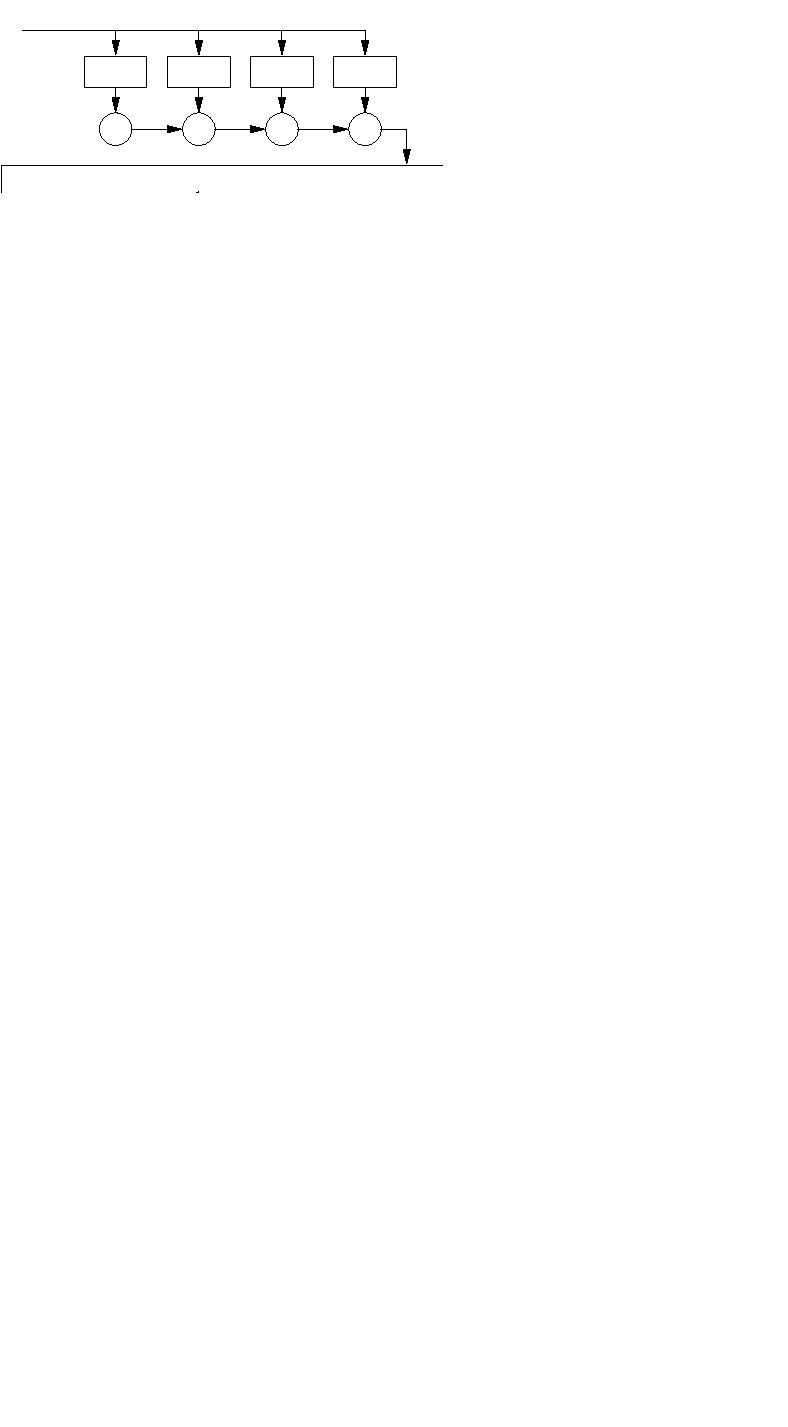
\includegraphics{pre_reverb_serial_des.pdf}%
\end{picture}%
\setlength{\unitlength}{3646sp}%
%
\begingroup\makeatletter\ifx\SetFigFont\undefined%
\gdef\SetFigFont#1#2#3#4#5{%
  \reset@font\fontsize{#1}{#2pt}%
  \fontfamily{#3}\fontseries{#4}\fontshape{#5}%
  \selectfont}%
\fi\endgroup%
\begin{picture}(6819,12342)(-3156,-5764)

\put(-314,4934){$x_1[n]$}%
\put(-3464,6419){$x[n]$}%
\put(-1439,5879){$z^{-ed_3}$}%
\put(-719,5879){$z^{-ed_4}$}%
\put(-2744,5384){$\Sigma$}%
\put(-2024,5384){$\Sigma$}%
\put(-1304,5384){$\Sigma$}%
\put(-2159,5879){$z^{-ed_2}$}%
\put(-2879,5879){$z^{-ed_1}$}%
\put(-584,5384){$\Sigma$}%

\end{picture}%
  \caption{Part of the Block diagram of a \gls{reverb} unit.}
  \label{fig:pre_reverb_block_design}
\end{figure}

\subsection{The \textit{reverb_lpcf} Subroutine}